\iflanguage{english}
{\chapter{Appendix}}    % english style
{\chapter{Anhang}}      % german style
\label{chap:appendix}

%%%%%%%%%% Uniqueness distribution %%%%%%%%%%%%
\begin{figure}[!htb]
     \centering
     
     \begin{subfigure}{0.49\textwidth}
         \centering
         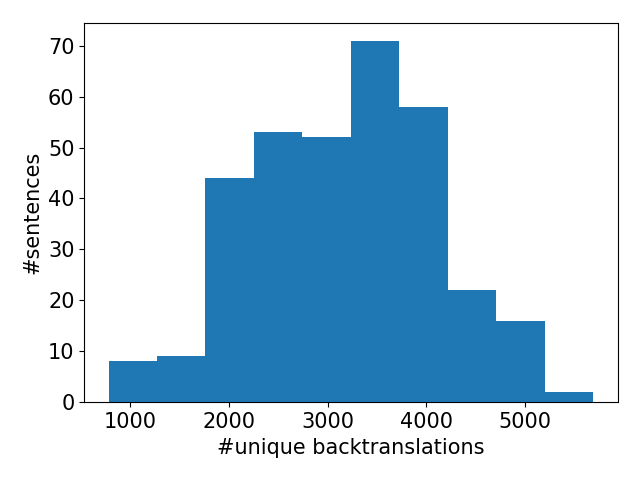
\includegraphics[width=\textwidth]{figures/uniqueness/unique_beam100/unique_back_original.png}
         \caption{Ambiguous Subset}
         %\label{fig:uniqueness_ambiguous}
     \end{subfigure}
     \hfill
     \begin{subfigure}{0.49\textwidth}
         \centering
         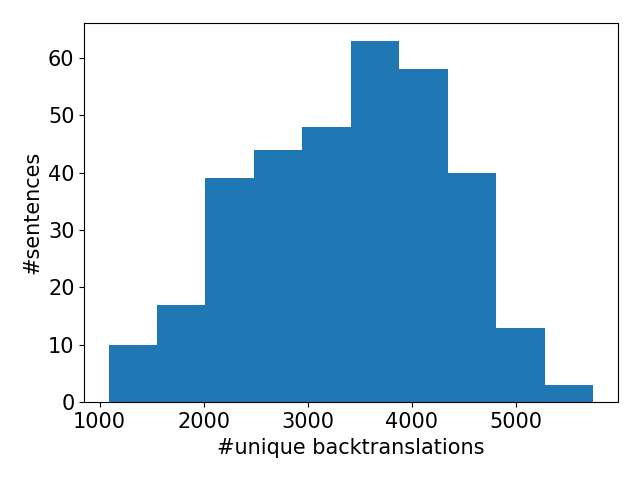
\includegraphics[width=\textwidth]{figures/uniqueness/unique_beam100/unique_back_male.png}
         \caption{Disambiguated Subset (male)}
         %\label{fig:uniqueness_male}
     \end{subfigure}
     \begin{subfigure}{0.49\textwidth}
         \centering
         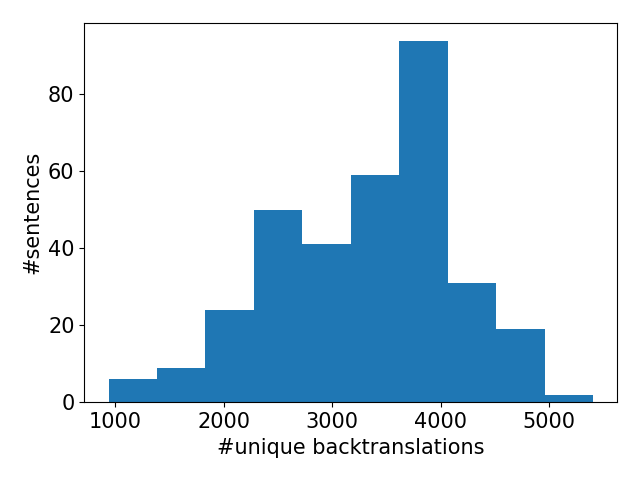
\includegraphics[width=\textwidth]{figures/uniqueness/unique_beam100/unique_back_average.png}
         \caption{Non-ambiguous Subset Average}
         %\label{fig:uniqueness_common}
     \end{subfigure}
     \hfill
     \begin{subfigure}{0.49\textwidth}
         \centering
         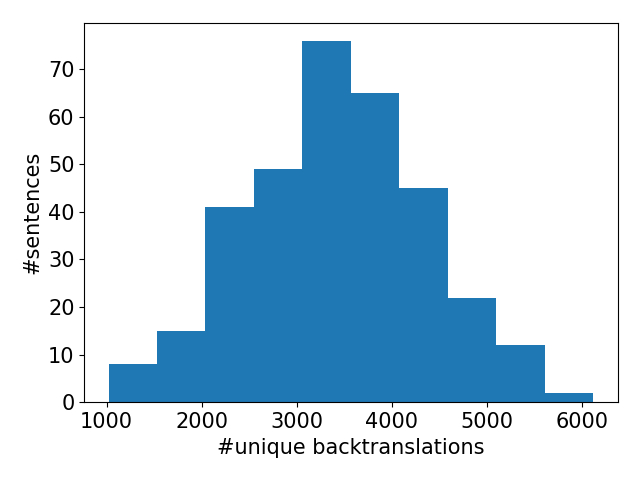
\includegraphics[width=\textwidth]{figures/uniqueness/unique_beam100/unique_back_female.png}
         \caption{Disambiguated Subset (female)}
         %\label{fig:uniqueness_female}
     \end{subfigure}
        \caption{Distribution of Unique Backtranslations: Beam search with beam size 100}
        \label{fig:uniqueness_graphs_100}

\end{figure}

\begin{figure}[!htb]
     \centering
     
     \begin{subfigure}{0.49\textwidth}
         \centering
         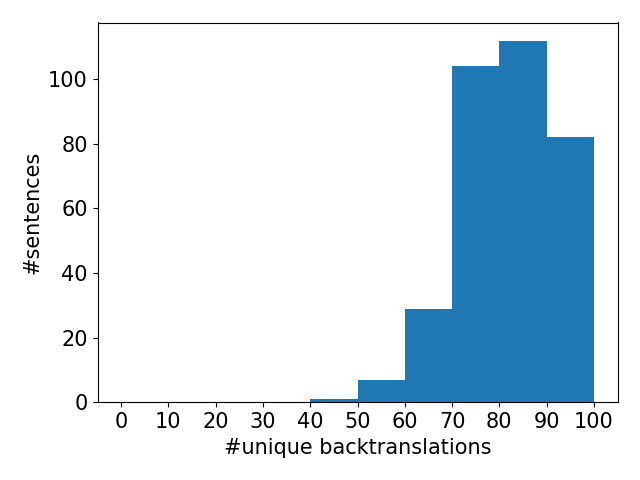
\includegraphics[width=\textwidth]{figures/uniqueness/unique_sampling/unique_back_original.png}
         \caption{Ambiguous Subset}
         %\label{fig:uniqueness_ambiguous}
     \end{subfigure}
     \hfill
     \begin{subfigure}{0.49\textwidth}
         \centering
         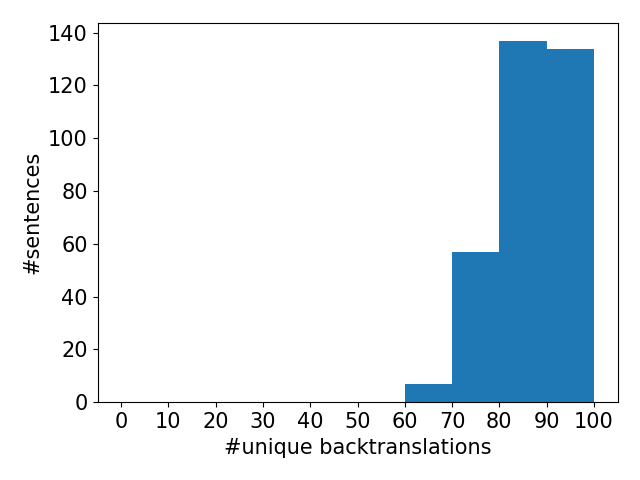
\includegraphics[width=\textwidth]{figures/uniqueness/unique_sampling/unique_back_male.png}
         \caption{Disambiguated Subset (male)}
         %\label{fig:uniqueness_male}
     \end{subfigure}
     \begin{subfigure}{0.49\textwidth}
         \centering
         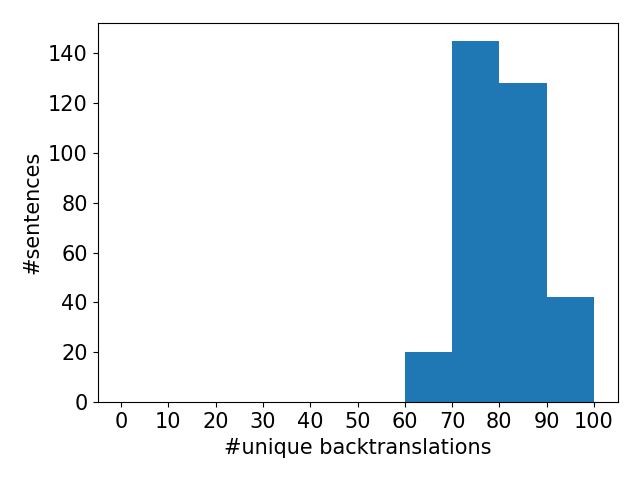
\includegraphics[width=\textwidth]{figures/uniqueness/unique_sampling/unique_back_average.png}
         \caption{Non-ambiguous Subset Average}
         %\label{fig:uniqueness_common}
     \end{subfigure}
     \hfill
     \begin{subfigure}{0.49\textwidth}
         \centering
         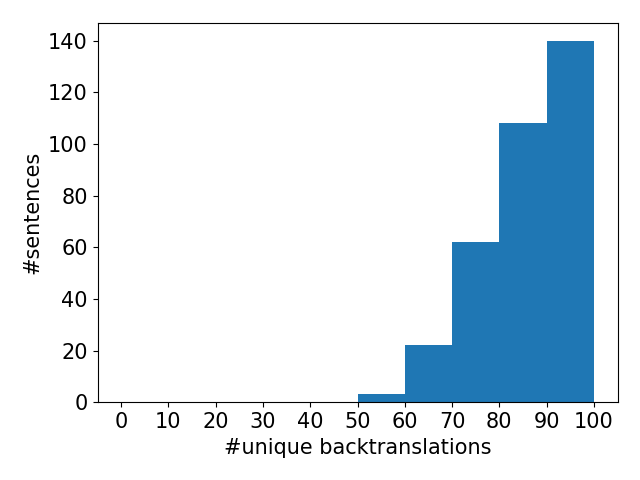
\includegraphics[width=\textwidth]{figures/uniqueness/unique_sampling/unique_back_female.png}
         \caption{Disambiguated Subset (female)}
         %\label{fig:uniqueness_female}
     \end{subfigure}
        \caption{Distribution of Unique Backtranslations: Sampling}
        \label{fig:uniqueness_graphs_sampling}

\end{figure}


%%%%%%%%%% Alignment distribution %%%%%%%%%%%%

% Beam 100
% Distribution for Translation
\begin{figure}[!htb]
     \centering
     
     \begin{subfigure}{0.49\textwidth}
         \centering
         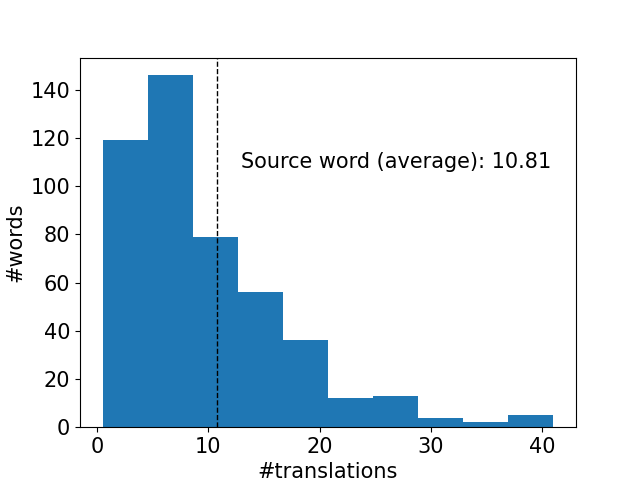
\includegraphics[width=\textwidth]{figures/alignment/align_100/word_translations_original.png}
         \caption{Ambiguous Subset}
         %\label{fig:alignment_translation_ambiguous}
     \end{subfigure}
     \hfill
     \begin{subfigure}{0.49\textwidth}
         \centering
         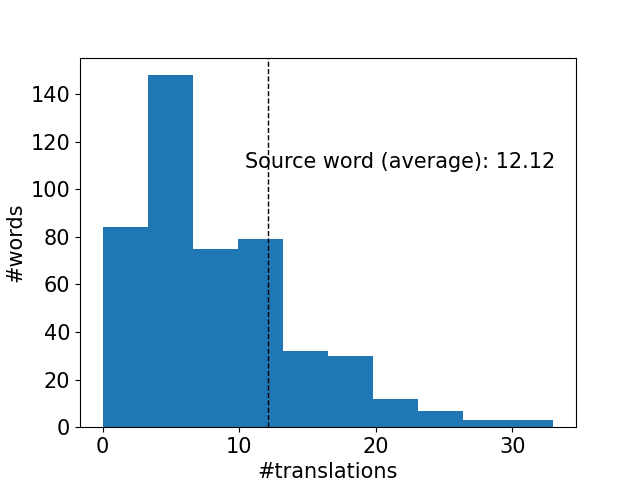
\includegraphics[width=\textwidth]{figures/alignment/align_100/word_translations_male.png}
         \caption{Disambiguated Subset (male)}
         %\label{fig:alignment_translation_male}
     \end{subfigure}
     \begin{subfigure}{0.49\textwidth}
         \centering
         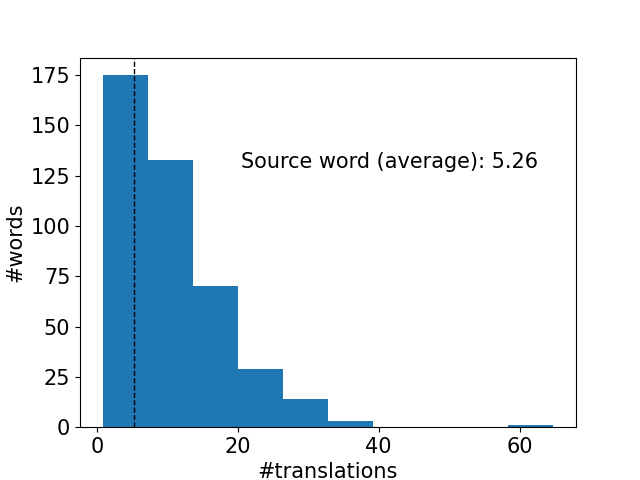
\includegraphics[width=\textwidth]{figures/alignment/align_100/word_translations_average.png}
         \caption{Non-ambiguous Subset Average}
         %\label{fig:alignment_translation_common}
     \end{subfigure}
     \hfill
     \begin{subfigure}{0.49\textwidth}
         \centering
         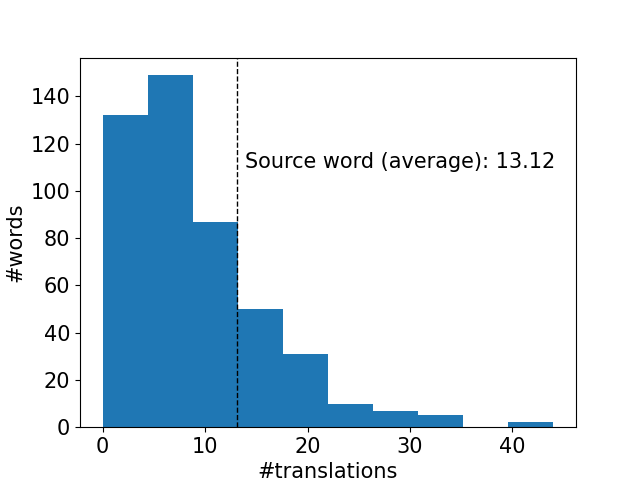
\includegraphics[width=\textwidth]{figures/alignment/align_100/word_translations_female.png}
         \caption{Disambiguated Subset (female)}
         %\label{fig:alignment_translation_female}
     \end{subfigure}
        \caption{\textbf{Distribution of Unique Translations for Words}. Beam search with beam size 100. Nbest size 100. Alignment with \textit{awesome-align}. The dashed line marks the average number of unique translations for the source word, the value displayed to the right.}
        \label{fig:alignment_graphs_translation_100}

\end{figure}

% Distribution for Backtranslation
\begin{figure}[!htb]
     \centering
     
     \begin{subfigure}{0.49\textwidth}
         \centering
         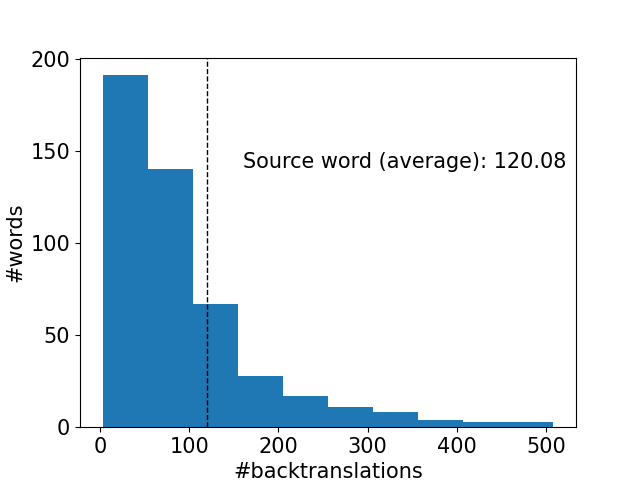
\includegraphics[width=\textwidth]{figures/alignment/align_100/word_backtranslations_original.png}
         \caption{Ambiguous Subset}
         %\label{fig:alignment_backtranslation_ambiguous}
     \end{subfigure}
     \hfill
     \begin{subfigure}{0.49\textwidth}
         \centering
         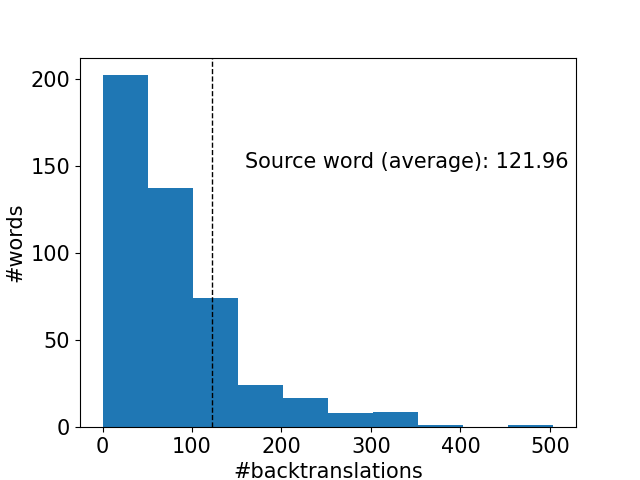
\includegraphics[width=\textwidth]{figures/alignment/align_100/word_backtranslations_male.png}
         \caption{Disambiguated Subset (male)}
         %\label{fig:alignment_backtranslation_male}
     \end{subfigure}
     \begin{subfigure}{0.49\textwidth}
         \centering
         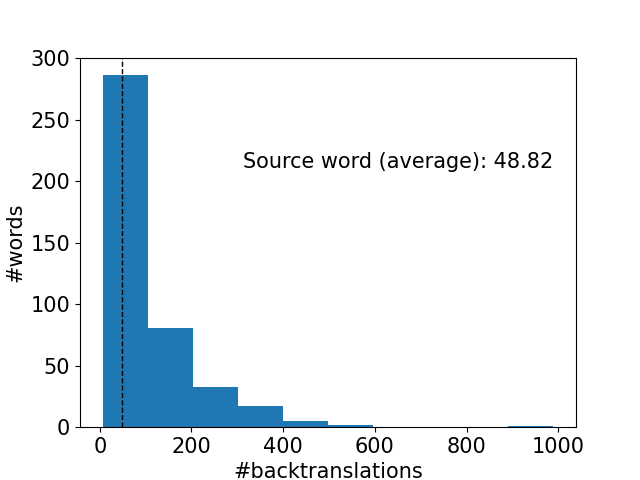
\includegraphics[width=\textwidth]{figures/alignment/align_100/word_backtranslations_average.png}
         \caption{Non-ambiguous Subset Average}
         %\label{fig:alignment_backtranslation_common}
     \end{subfigure}
     \hfill
     \begin{subfigure}{0.49\textwidth}
         \centering
         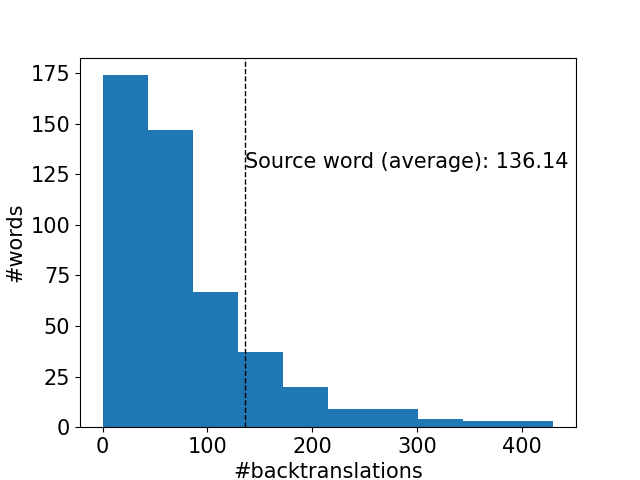
\includegraphics[width=\textwidth]{figures/alignment/align_100/word_backtranslations_female.png}
         \caption{Disambiguated Subset (female)}
         %\label{fig:alignment_backtranslation_female}
     \end{subfigure}
        \caption{\textbf{Distribution of Unique Backtranslations for Words}. Beam search with beam size 100. Nbest size 100. Alignment with \textit{awesome-align}. The dashed line marks the average number of unique translations for the source word, the value displayed to the right.}
        \label{fig:alignment_graphs_backtranslation_100}

\end{figure}

% Sampling
% Distribution for Translation
\begin{figure}[!htb]
     \centering
     
     \begin{subfigure}{0.49\textwidth}
         \centering
         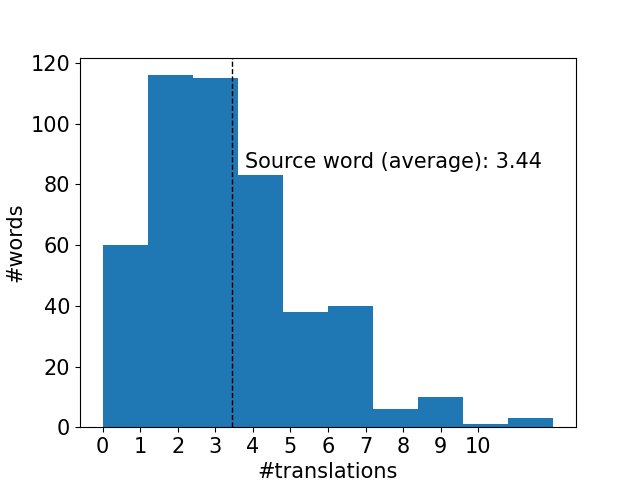
\includegraphics[width=\textwidth]{figures/alignment/align_sampling/word_translations_original.png}
         \caption{Ambiguous Subset}
         %\label{fig:alignment_translation_ambiguous}
     \end{subfigure}
     \hfill
     \begin{subfigure}{0.49\textwidth}
         \centering
         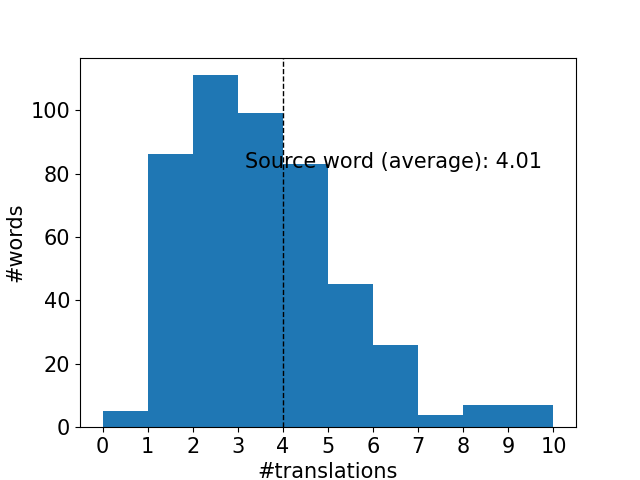
\includegraphics[width=\textwidth]{figures/alignment/align_sampling/word_translations_male.png}
         \caption{Disambiguated Subset (male)}
         %\label{fig:alignment_translation_male}
     \end{subfigure}
     \begin{subfigure}{0.49\textwidth}
         \centering
         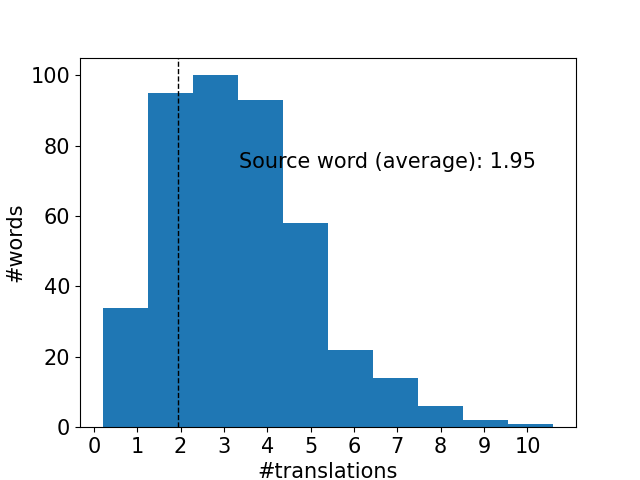
\includegraphics[width=\textwidth]{figures/alignment/align_sampling/word_translations_average.png}
         \caption{Non-ambiguous Subset Average}
         %\label{fig:alignment_translation_common}
     \end{subfigure}
     \hfill
     \begin{subfigure}{0.49\textwidth}
         \centering
         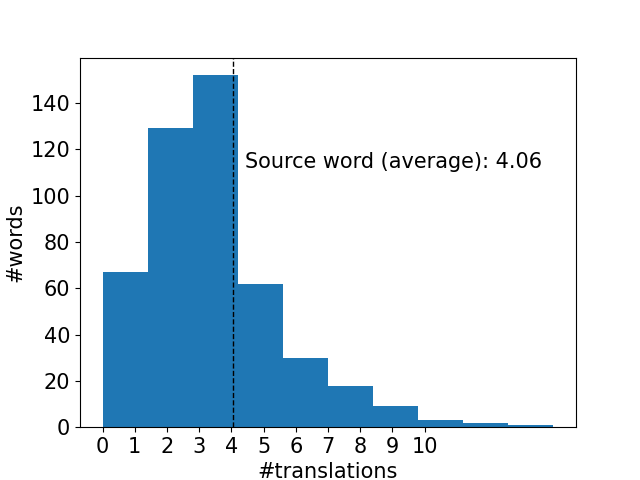
\includegraphics[width=\textwidth]{figures/alignment/align_sampling/word_translations_female.png}
         \caption{Disambiguated Subset (female)}
         %\label{fig:alignment_translation_female}
     \end{subfigure}
        \caption{\textbf{Distribution of Unique Translations for Words}. Sampling. Nbest size 10. Alignment with \textit{awesome-align}. The dashed line marks the average number of unique translations for the source word, the value displayed to the right.}
        \label{fig:alignment_graphs_translation_sampling}

\end{figure}

% Distribution for Backtranslation
\begin{figure}[!htb]
     \centering
     
     \begin{subfigure}{0.49\textwidth}
         \centering
         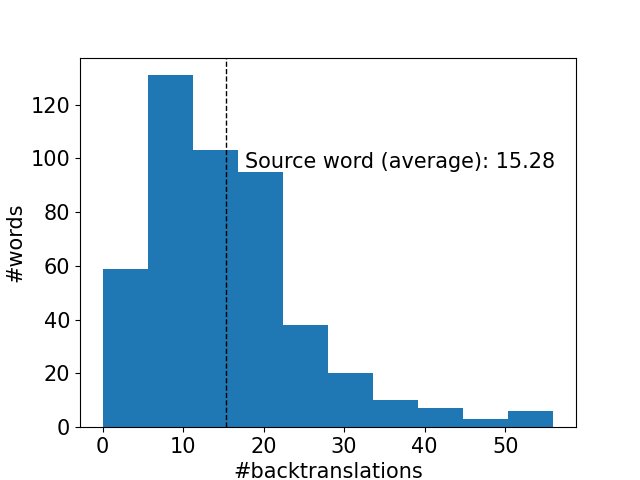
\includegraphics[width=\textwidth]{figures/alignment/align_sampling/word_backtranslations_original.png}
         \caption{Ambiguous Subset}
         %\label{fig:alignment_backtranslation_ambiguous}
     \end{subfigure}
     \hfill
     \begin{subfigure}{0.49\textwidth}
         \centering
         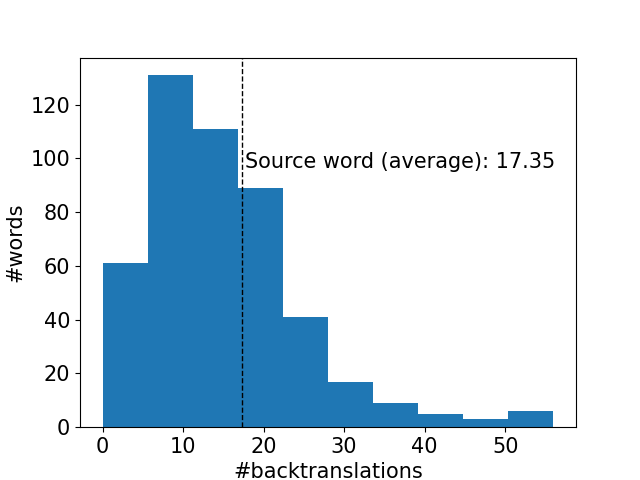
\includegraphics[width=\textwidth]{figures/alignment/align_sampling/word_backtranslations_male.png}
         \caption{Disambiguated Subset (male)}
         %\label{fig:alignment_backtranslation_male}
     \end{subfigure}
     \begin{subfigure}{0.49\textwidth}
         \centering
         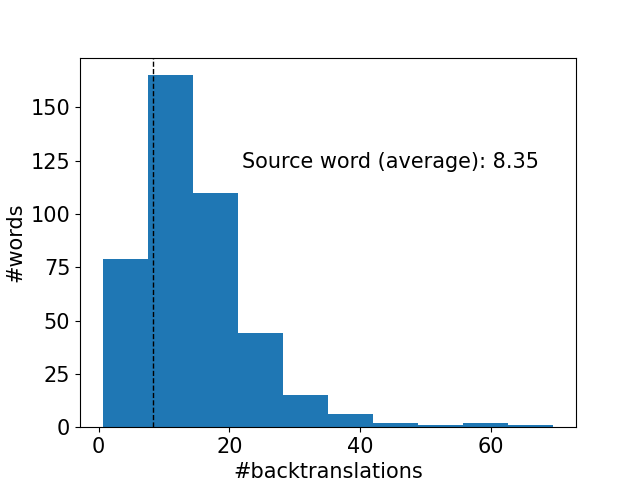
\includegraphics[width=\textwidth]{figures/alignment/align_sampling/word_backtranslations_average.png}
         \caption{Non-ambiguous Subset Average}
         %\label{fig:alignment_backtranslation_common}
     \end{subfigure}
     \hfill
     \begin{subfigure}{0.49\textwidth}
         \centering
         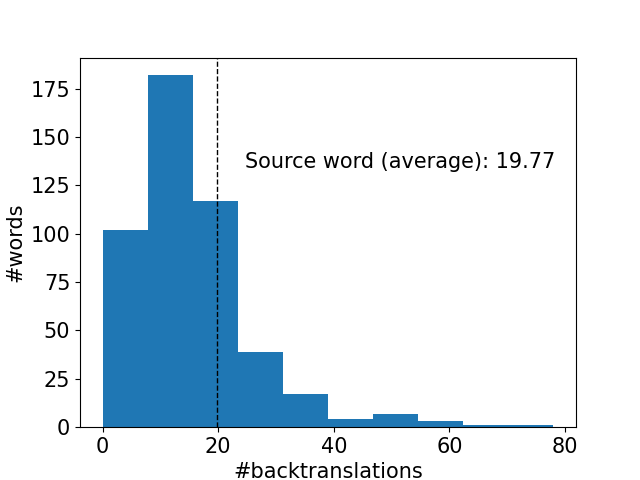
\includegraphics[width=\textwidth]{figures/alignment/align_sampling/word_backtranslations_female.png}
         \caption{Disambiguated Subset (female)}
         %\label{fig:alignment_backtranslation_female}
     \end{subfigure}
        \caption{\textbf{Distribution of Unique Backtranslations for Words}. Sampling. Nbest size 10. Alignment with \textit{awesome-align}. The dashed line marks the average number of unique translations for the source word, the value displayed to the right.}
        \label{fig:alignment_graphs_backtranslation_sampling}

\end{figure}